\chapter{Directed motion of metallodielectric particles by contact charge electrophoresis}
%%%%%%%%%%%%%%%%%%%%%%%%%%%%%%
\section{Introduction}\footnotetext{This chapter is adapted from  Dou, Yong, et al. "Directed motion of metallodielectric particles by contact charge electrophoresis." Langmuir 32.49 (2016): 13167-13173. }

Self-propelled colloidal particles harness energy from their environment to power directed motions relative to their fluid surroundings \cite{ebbens2016active,Li2016,Dey2016}.
Inspired by the locomotion of micro-organisms \cite{Lauga2009}, these artificial swimmers are actively pursued for their potential to navigate complex environments \cite{Takagi2014,Das2015} and deliver cargo to targeted locations\cite{Gao2015,Baylis2015}.
Fluid flows induced by particle motions can also serve to enhance rates of mass transfer to/from the particle surface with emerging applications in water remediation\cite{Soler2013,Li2014} and chemical detection\cite{morales2014micromotor,kagan2009chemical}.
When many self-propelled particles get together, they often interact to form dynamic assemblies\cite{Wang2015} such as swarms\cite{Ibele2009,Nguyen2012}, flocks \cite{Bricard2013}, clusters\cite{JieZhang2016}, and crystals \cite{Palacci2013}.
Synthetic realizations of such active matter\cite{Marchetti2013} provide useful models by which to explore the many forms of self-organization that arise outside of thermodynamic equilibrium.
Importantly, the diverse behaviors of motile particles depend critically on the specific mechanism of self-propulsion and on the associated interactions among the particles.
Expanding the repertoire of colloidal self-propulsion can therefore enable the discovery of new dynamical behaviors as well as the development of future applications.

A wide variety of physicochemical mechanisms have been applied to power the self-propulsion of colloidal particles.
Self-phoretic mechanisms\cite{Golestanian2007} use asymmetries in particle shape and/or composition to create local gradients in the electric potential\cite{Brown2014}, chemical composition\cite{Howse2007}, or temperature\cite{Jiang2010} that drive particle motions via interfacial phoretic effects such as electrophoresis, diffusiophoresis, or thermophoresis, respectively\cite{Anderson1989}.
In a classic example\cite{Paxton2004,Fournier-Bidoz2005}, bimetallic nanorods move autonomously through a homogeneous liquid containing a suitable chemical fuel via reaction-induced  self-electrophoresis\cite{Wang2006,Moran2010}. 
Self-propelled motions of asymmetric particles can also be powered by external fields.
Alternating electric fields drive motions of polarizable particles by induced charge electrophoresis \cite{Squires2006,Gangwal2008,Boymelgreen2014}; alternating magnetic fields power the swimming of flexible magnetic particles by inducing non-reciprocal beating motions \cite{Dreyfus2005}; acoustic fields propel dense metallic particles by directing steady streaming flows\cite{Wang2012,Nadal2014,Ahmed2015}. 
These examples of field-driven particle motion are generally considered forms of self-propulsion, as they allow particles to move freely in multiple directions (typically those perpendicular to the applied field).
The use of external fields to power such motions is attractive for studies of active matter as their magnitude is tunable in space and time.

Here, we describe a type of colloidal self-propulsion in which an electric field drives the autonomous motion of metallodielectric Janus particles\cite{Perro2005,Pawar2008} within an insulating liquid between two plane electrodes (Fig.~\ref{fig:1}a).
Similar configurations have been used to investigate particle motions powered by induced charge electrophoresis within conductive liquids\cite{Boymelgreen2014} and by Quicke rotation within weakly conductive liquids \cite{Bricard2013}.
By contrast, field-driven  motion of conductive particles in insulating liquids is driven by contact charge electrophoresis (CCEP) whereby particles acquire charge on contact with a biased electrode and then move in the field emanating from that electrode \cite{drews2013ratcheted,cartier2014microfluidic,drews2015contact}.
In one well studied example, a conductive sphere immersed in mineral oil oscillates rapidly between two electrodes subject to a constant voltage \cite{drews2015contact}.
Each time the particle contacts an electrode, it acquires charge of opposite polarity and moves back towards the other electrode thereby transporting charge down the applied potential gradient.
Harnessing these motions for useful functions requires strategies by which to rectify particle oscillations.
One approach is to modify the electrodes with asymmetric, ratchet-like features that enable directed transport of conductive particles\cite{drews2013ratcheted} or droplets\cite{Um2016}.
Here, we introduce an alternative strategy that relies on particle asymmetries to achieve similar directed motions.

We show that oscillations of Janus particles between two parallel electrodes are accompanied by steady motions directed perpendicular to the applied field.
Through experiment and theory, we develop and validate a mechanism of self-propulsion whereby the field-induced rotation of the particle upon charge reversal at the electrode surface results in its net displacement during each oscillation cycle.
Repeated displacements in a common direction propel Janus particles at speeds of up to $600~\mu\text{m/s}$ along wide circular arcs within the plane of the electrodes.
Beyond the dynamics of individual particles, we show how particles can both attract or repel one another depending on their separation and on the phases of their respective oscillations.
Together, these results demonstrate how particle symmetry can be used to direct the motions of active colloids powered by CCEP.
The ability to engineer the motions of individual particles and their assemblies will ultimately contribute to the realization of colloidal machines that organize and operate autonomously to perform useful functions \cite{Spellings2015}.

\begin{figure}[p]
\centering
\includegraphics[width=9cm]{figures/2_1.pdf}
\caption{ (a) Schematic illustration of the experimental setup. A metallodieletric Janus particle is immersed in mineral oil between two parallel ITO electrodes (left).  Application of a constant voltage $V$ results in the oscillatory motion of the particle via contact charge electrophoresis (CCEP; right). (b) When imaged from above, the particle moves in and out of focus in time as it oscillates between the electrodes. (c) Over many oscillation cycles, the particle moves steadily away from its conductive hemisphere (top); the steady motion of the particle continues over hundreds of microns (bottom).  See supporting videos 1, 2, and 3.}
\label{fig:1}
\end{figure}
 
 
%%%%%%%%%%%%%%%%%%%%%%%%%%%%%%
\section{Experimental Section}

In a typical experiment, a dilute suspension of Janus particles in mineral oil was sandwiched between two parallel  electrodes separated by a distance $H= 50 - 250~\mu\text{m}$ (Fig.~\ref{fig:1}a). 
We used two types of Janus particles: $8~\mu\text{m}$ silica particles and $4~\mu\text{m}$ fluorescent polystyrene particles, each coated on one hemisphere by a thin layer of gold.
In the absence of an applied field, the particles settled to the surface of the lower electrode where they were imaged from above by an optical microscope.
Application of a constant voltage $V = 200 - 1000~\text{V}$ caused the particles to oscillate rapidly between the electrodes, as evidenced by their periodic appearance and disappearance from the focal plane (Fig.~\ref{fig:1}b). 
Each time a particle came into focus, its position was displaced slightly from that in the previous cycle.
The magnitude and direction of these displacements was relatively constant from one cycle to the next resulting in steady particle motions perpendicular to the applied field.
Using high speed imaging, we quantified the frequency $f$ of particle oscillations as well as the particle position $(x_p,y_p)$ at each oscillation cycle.
For example, at $V = 400~\text{V}$ and $H=200~\mu\text{m}$, a silica Janus particle oscillated between the electrodes at an average frequency of $f = 29~\text{Hz}$ and moved perpendicular to the field at an average speed of $U_{\perp} = 25~\mu\text{m/s}$ (Fig.~\ref{fig:1}c).
Directed particle motion continued over large distances for as long as the voltage was applied.

\subsection{Synthesis of Janus Particles}

Silica Janus particles were prepared by  deposition of gold onto particle monolayers supported on glass slides.
Following Prevo and Velev \cite{prevo2004controlled}, $10~\mu\text{L}$ of a concentrated (30 wt\%) suspension of $8~\mu\text{m}$ silica particles in water was placed between two acid-cleaned microscope slides mounted at an angle on a motorized stage (Harvard Apparatus PHD 2000).
The trapped colloidal solution was dragged at a prescribed speed by the motion of the top slide to achieve well-packed monolayers.
Successive layers of metal (5 nm Ti and 10 nm Au) were then deposited by physical vapor deposition (Cressington 308).

Fluorescent Janus particles were prepared following a procedure adapted from Kopelman et al. \cite{Sinn2011}.
Briefly, sulfonated fluorescent polystyrene particles (ThermoFisher F8858) were washed three times in water by centrifugation and dispersed in methanol at a concentration of 1\% w/v. 
0.5 ml of the particle suspension was deposited onto a 4-inch silicon wafer wafer by spin coating at 2500 rpm for 15 second. 
Successive layers of metal (5 nm Ti, 25 nm Ni, and 20 nm Au) were then deposited by e-beam evaporation (Kurt J Lesker Co. Lab 18). 
The nickel layer was included for a purpose unrelated to the present experiments and is unnecessary here. 
The particles were gently brushed off the wafer using a damp brush.

\subsection{Electrode Configuration}

The electrode setup was comprised of two transparent  indium tin oxide (ITO)-coated glass slides (SIGMA-Aldrich, CAS:50926-11-9, surface resistivity 70-100 $\Omega$/sq) separated from one another by spacers made of glass ($150~\mu\text{m}$ to $250~\mu\text{m}$ thick cover slides) or polydimethylsiloxane (PDMS, $50~\mu\text{m}$ to $100~\mu\text{m}$ thick).
The ITO electrodes were connected to a high-voltage source (Keithley 2410) with a limiting current of $10~\mu\text{A}$ to prevent damage to the system in the event of a short-circuit.
The Janus particles were dispersed in Nylon membrane-filtered mineral oil (SIGMA-Aldrich, CAS:8042-47) at a concentration of $0.01-1~\text{mg/ml}$ and injected into the inter-electrode region.
We note that the charge relaxation time for mineral oil is considerably larger the the timescale of particle oscillations, which is a necessary condition for CCEP \cite{cartier2014microfluidic}. 
The field-induced motion of the Janus particles was captured by a high speed camera (Phantom V310) mounted on an optical microscope (Zeiss Axio Imager A1) operating in bright field mode with 10x and 50x objectives.

\subsection{Particle Tracking}

Movies were captured at frame rates of 1,000 -- 5,000 fps and processed in MATLAB to analyze particle oscillations and reconstruct particle trajectories. 
To determine the oscillation frequency, we first identified a fixed window around a single particle and computed the window-averaged pixel intensity for each frame.
This average intensity oscillated in time as the particle moved into and out of focus, reaching its local minimal value when the particle came into focus at the lower electrode.
For each oscillation cycle $i=1,2,\dots, N$, we identified the time $t_i$ when the particle contacted the lower electrode. 
The mean oscillation frequency was then computed by dividing the number of particle oscillations by the total observation time, $f= N / (\Sigma_i t_i)$.
To reconstruct particle trajectories $(x_i,y_i)$, we considered only those frames when the particle was in focus (i.e., when the average intensity was in local minimum) and determined the location of the particle center using standard algorithms \cite{Track}.
The net displacement for cycle $i$ was computed as $\Delta_i^2 = (x_{i+1} - x_i)^2 + (y_{i+1}-y_i)^2$; the average speed of the particle (parallel to the electrodes) was computed as $U_{\perp} = (\Sigma_i \Delta_i)  /  (\Sigma_i t_i$).

\subsection{Simulation of CCEP Motions}

The model of CCEP dynamics combines classical electrostatics and low Reynolds number hydrodynamics \cite{drews2015contact}. 
The metallic hemisphere of the Janus particle as well as the bounding electrodes are treated as perfect conductors.
To facilitate our numerical analysis, the conductive portion of the particle is modeled as a solid hemisphere with rounded corners (radius $0.1a$) in contrast to the thin hemispherical cap present in experiment.
Additionally, the non-metallic hemisphere and the surrounding fluid are assumed to be dielectrics with a common permittivity $\varepsilon$.
Given the particle charge $q$, orientation $\alpha$, and height $z_p$ above the electrode surface, we solve the Laplace equation numerically to determine the electric potential $\Phi$ and field $\ve{E}=-\nabla \Phi$ throughout the dielectric medium (see Supporting Information for details).
We then integrate the Maxwell stress over the surface of the conductive hemisphere to determine the electric force and torque that drive particle motion.

At low Reynolds numbers (in experiments $Re\leq0.01$), the translational and rotational velocities of the particle are linearly related to the external force and torque by the so-called resistance tensor \cite{Kim2005, Swan2007}.
For a spherical particle near a solid plane boundary, there exist exact analytical expressions \cite{Kim2005} for the components of this tensor, which, when suitably rescaled, depends only on the separation between the sphere and the plane. 
Using these expressions, we compute the particle velocity and integrate numerically to determine the position and orientation of the particle as a function of time.
We assume that the charge $q$ on the particle remains constant until the surface of the metallic hemisphere reaches some critical separation $\delta$ from the plane electrode, at which point charge flows to/from the particle instantaneously to reverse the particle polarity ($q\rightarrow -q$).
Physically, the contact charging process is thought to occur by a type of dielectric breakdown; the resulting charge on the particle is somewhat variable but consistently less than that expected at equilibrium (i.e., when the potential on the particle equals that of the electrode) \cite{drews2015contact}.
After nondimensionalization, the computed particle trajectories depend on just two parameters: the dimensionless charge $q / 4\pi\varepsilon a^2 E$ and the dimensionless separation at contact $\delta / a$.


%%%%%%%%%%%%%%%%%%%%%%%%%%%%%%
\section{Results and Discussion}

Figure \ref{fig:2}a shows the reconstructed trajectories of six different Janus particles under identical conditions over the course of one hundred oscillation cycles based on the experiment results. 
The cumulative displacement of each particle increased roughly linearly with the number of oscillations (Fig.~\ref{fig:2}b) as the particles moved along wide circular arcs of radius $30~\mu\text{m}$ or greater.
These observations are consistent with the spatial homogeneity of the applied field, which suggests that particle motion be invariant to translation and rotation in the $xy$ plane of the electrodes.
Although the majority of particles (ca.~70\% for $V=800~\text{V}$ and $H=200~\mu\text{m}$) exhibited such directed motions, some Janus particles were observed to oscillate between the electrodes with no lateral motion whatsoever.
Additionally, some particles (ca.~20\%) remained ``stuck'' to the electrode surface and did not move at all upon application of the field.

For the particles that moved, the oscillation frequency increased monotonically with increasing voltage as $f \propto V^{2}$ (Fig.~\ref{fig:2}c).
This observation is consistent with previous studies of CCEP motion, which showed that the oscillation frequency scales as $f\sim\varepsilon a V^2 / \eta H^3$, where $\varepsilon$ and $\eta$ are the permittivity and viscosity of the fluid, respectively, and $a$ is the particle radius \cite{drews2015contact}.
By contrast, the lateral displacement of the particle during each oscillation cycle was largely independent of the applied voltage; each oscillation contributed an average displacement of $\Delta = 0.2 a$ (Fig.~\ref{fig:2}d).
Consequently, the lateral velocity of the particle, $U_{\perp}\equiv f\Delta$, also increased as the square of the applied voltage (Fig.~\ref{fig:2}e).
This velocity could be further increased by decreasing the spacing between the electrodes $H$ to increase the magnitude of the applied field (Fig.~\ref{fig:2}f). 
Using spacers of $H=50~\mu\text{m}$, we observed particles velocities up to $U_{\perp}=600~\mu\text{m/s}$ in the direction perpendicular to the applied field.


\begin{figure}[p]
\centering
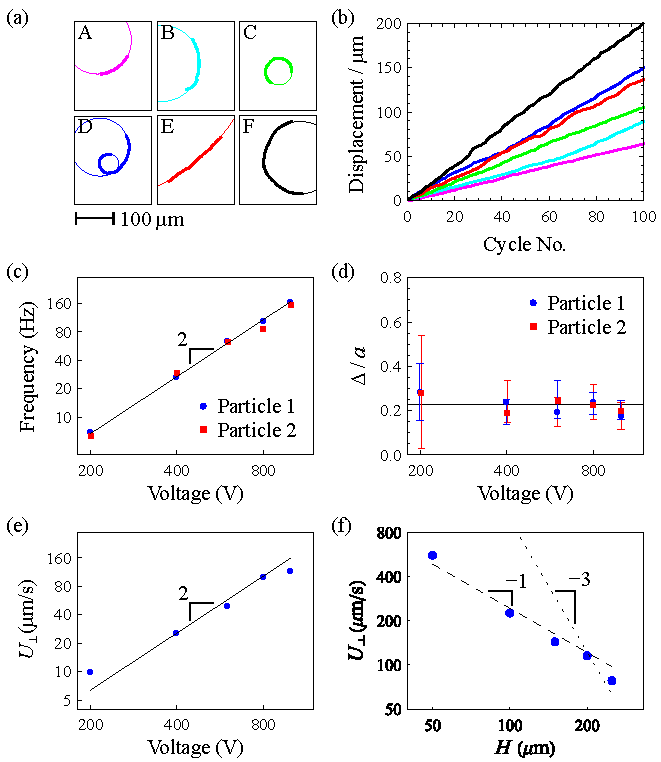
\includegraphics[width=11.2cm]{figures/2_2.pdf}
\caption{(a) Reconstructed particle trajectories of six Janus particles (radius $a = 4~\mu\text{m}$; voltage $V=800~\text{V}$; electrode spacing $H=200~\mu\text{m}$).  Markers denote the particle position at successive oscillations; curves are best circular fits to the data. (b) The cumulative displacement of particles in (a) increases linearly with the number of oscillation cycles. (c) The oscillation frequency of the particle scales quadratically with the voltage.  Markers show data for two independent particles with an electrode spacing $H=200~\mu\text{m}$; the curve is a fit of the form $f\propto V^2$. (d) The lateral particle  displacement $\Delta$ during each oscillation is largely independent of the applied voltage. Markers show the mean displacement; error bars denote one standard deviation above and below the mean. (e) The particle velocity perpendicular to the field scales as the square of the voltage. Markers show data for one particle with an electrode spacing $H=200~\mu\text{m}$; the curve is a fit of the form $U_{\perp}\propto V^2$. (f) Particle velocity increases with decreasing electrode spacing. Each marker represents the velocity of a single particle for an applied voltage $V=800~\text{V}$.}
\label{fig:2}
\end{figure}

To explain these experimental observations, we propose the following propulsion mechanism illustrated in Figure \ref{fig:3}a. 
As it moves across the channel, a charged Janus particle adopts a preferred orientation in which its principal axis is oblique to the applied field and its motion is directed towards the metallic hemisphere.
When it contacts either electrode, the charge on the particle changes sign thereby altering its preferred orientation in the field.
The field-induced rotation of the particle in the vicinity of the electrode surface results in a lateral displacement, which is qualitatively similar to that of a sphere ``rolling'' along the surface.
Successive rotations occur in a common direction towards the non-metallic hemisphere causing a steady lateral motion over the course of many oscillations.
This putative mechanism is supported both by experimental observations of the transient particle orientation and by a mathematical model that describes the electrostatics and hydrodynamics of CCEP motion.

\begin{figure}[p]
\centering
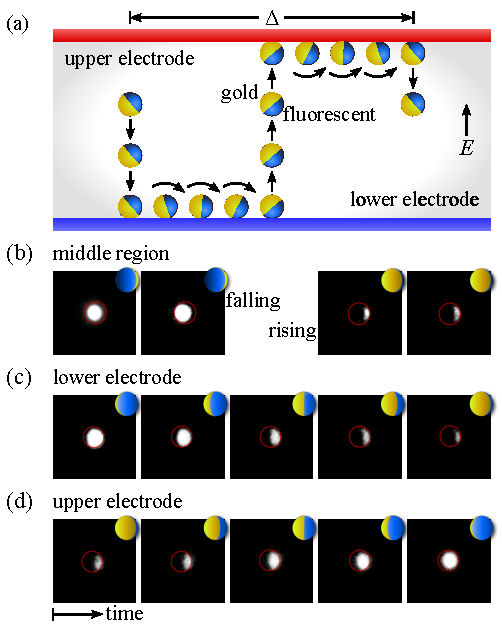
\includegraphics[width=8.5cm]{figures/2_3.pdf}
\caption{(a) Schematic illustration of the propulsion mechanism showing one oscillation cycle.  Rotation of the particle near the electrodes results in a lateral displacement $\Delta$. (b-d) Fluorescent microscopy images highlight the non-metallic hemispheres of fluorescent Janus particles. Images are captured from above; the icons show the particles viewed from above using the color scheme from (a). Particles in the middle region (b) adopt a stable orientation that depends on their direction of travel (falling vs.~rising). Upon contacting the lower (c) or upper (d) electrode, particles rotate in time from one orientation to another. See supporting video 4.}
\label{fig:3}
\end{figure}

We used fluorescent particles to better visualize the orientation of Janus particles moving by CCEP.  
Such particles appeared bright when the metallic hemisphere was directed ``down'' (negative $z$ direction; away from the microscope objective) and dark when the metallic hemisphere was directed ``up'' (positive $z$ direction; towards the objective). 
For intermediate orientations, the fluorescent hemisphere of the particle was partially visible like the bright side of the moon in different phases.
By focusing on planes in the middle of the two electrodes, we observed that particles moving downward appeared bright (gibbous moon) while those moving upward appeared dark (crescent moon) (Fig.~\ref{fig:3}b).
By focusing on the lower electrode, we directly observed the rotation of the particle as it transitioned from the gibbous to crescent configuration (Fig.~\ref{fig:3}c).  
The opposite behavior was observed at the upper electrode where the particle rotated from the crescent to gibbous configuration (Fig.~\ref{fig:3}d).
Importantly, the orientation of the Janus particle in the plane of the electrodes remained relatively constant from one cycle to the next, which allowed the particle to move steadily away from its metallic hemisphere.   

To gain further insights into the propulsion mechanism, we use the equations of classical electrostatics and low-Reynolds number hydrodynamics to describe the dynamical trajectories of Janus particles moving by CCEP.
We first consider the case of a single Janus particle with a net charge $q$ in an unbounded medium subject to a uniform electric field $E$.
We solve for the electric potential within the dielectric and evaluate the electrostatic torque $L(\alpha)$ on the particle as a function of its orientation $\alpha$ relative to the field.
For each charge, there exists one stable orientation for which the electric torque is zero $L(\alpha)=0$ and its derivative is negative $L'(\alpha)<0$ (Fig.~\ref{fig:4}a).
Uncharged Janus particles tend to orient perpendicular to the applied field owing to the increased polarizability of their metallic hemisphere in that orientation ($\alpha=\pi/2$ for $q=0$).
The addition of positive or negative charge, respectively, acts to rotate the particle towards or away from the direction of the field.
When the charge exceeds a critical magnitude, the particle orients perfectly with or against the applied field.
Importantly, this critical charge is similar in magnitude to that acquired by the particle during contact charging (see Fig.~S2). 

\begin{figure}[p]
\centering
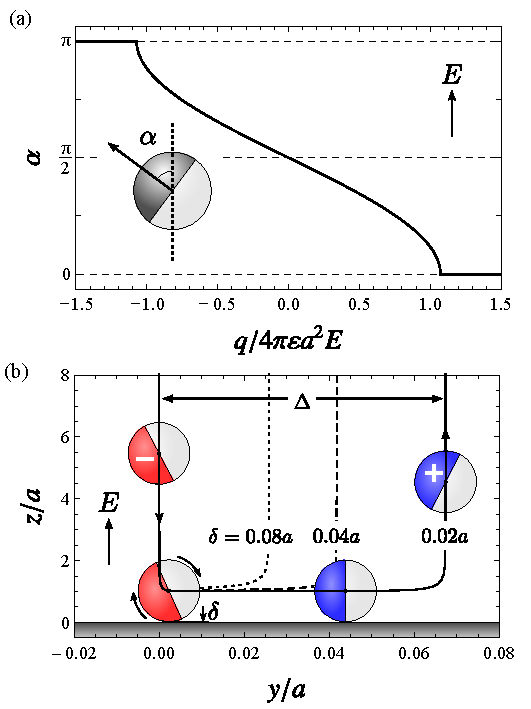
\includegraphics[width=9cm]{figures/2_4.pdf}
\caption{Results of the theoretical model. (a) The stable orientation $\alpha$ of a Janus particle in a uniform electric field depends on the particle's charge $q$ (scaled by $q_s = 4\pi\varepsilon a^2 E$). Uncharged particles align perpendicular to the applied field $E$ ($\alpha=\pi/2$ for $q=0$); highly charged particles align parallel to the field ($\alpha=0,\pi$ for $|q|>1.07 q_s$). (b) Simulated particle ``collisions'' with the lower electrode for a particle charge $q=\pm0.5q_s$. The solid curve shows the trajectory of the particle center; the orientation of the particle at different points along the trajectory is illustrated graphically. The net particle displacement $\Delta$ depends on the surface separation $\delta$ at contact when the particle charge reverses polarity. Note that for clarity the $z$ and $y$ axes use different scales.}
\label{fig:4}
\end{figure}

We now consider the dynamics of a particle ``collision'' with the lower electrode (Fig.~\ref{fig:4}b). 
Initially, the particle is positioned far from the electrode surface ($z_p\gg a$) with some fixed charge $q$. 
We solve for the electrostatic force and torque on the particle and compute the translational and rotational particle velocity in proximity to the surface.
We then integrate these dynamical equations of motion to describe the position and orientation of a single particle as function of time.
Figure \ref{fig:4}b shows three different particle trajectories for different contact separations and a common charge $q = 0.5 q_s$ where $q_s = 4\pi\varepsilon a^2 E$ is a convenient charge scale.
The trajectories are in qualitative agreement with the experimental observations: a particle moves towards the electrode with a preferred orientation, reverses its charge on contact, rotates and translates as it adopts a newly preferred orientation, and ultimately moves away from the surface.
The net lateral displacement $\Delta$ depends on how closely the particle approaches the surface.
For particles that approach more closely to the surface, their rotational motion is more tightly coupled to their lateral translation, and they move farther during each collision.
The displacement also depends on the particle charge in an somewhat surprising way: highly charged particles ($q > q_s$) exhibit little or no displacement (Fig.~S6).
Such particles contact the surface with their axis aligned parallel with field and therefore experience little or no torque upon charge reversal.
Instead, these particles move backward from the surface before ultimately rotating into the new stable orientation; particle rotation far from the surface, however, results in little or no lateral displacement.
This prediction of the model provides a plausible explanation for those particles that oscillate but do not translate perpendicular to the field.

There are some experimental observations that are not captured by the idealized model.
Notably, the model predicts that particles should move along straight lines and not the circular trajectories observed in experiment.
We attribute this discrepancy to defects on the Janus particles that break their axial symmetry.
Imperfections in the particles' metallic hemispheres are known to arise during metal deposition due to shadowing by neighboring particles \cite{Pawar2008}.
Such defects can lead to electric torques about the principle axis of the particle, which are otherwise prohibited by symmetry.
As a result, particles are permitted to change their orientation in the plane of the electrode upon charge reversal.
Understanding these effects requires further study of non-axisymmetric particles of well defined shape.
Interestingly, in some experiments, the curvature of the particle trajectory changed abruptly during its motion (e.g., particle D in Fig.~\ref{fig:2}a). 
This observation may imply that non-axisymmetric particles are capable of multiple ``modes'' of self-propulsion; however, we cannot yet dismiss alternative explanations based on adventurous dust particles.

As noted above, the propulsion velocity is equal to the product of the oscillation frequency and the rotation-induced displacement: $U_{\perp}=f\Delta$.
This expression suggests two basic strategies for maximizing the particle velocity: (i) increase the oscillation frequency, $f\sim\varepsilon a V^2/\eta H^3$, or (ii) increase the lateral displacement upon charge reversal.
The oscillation frequency can be enhanced by increasing the voltage or by decreasing the spacing between the electrodes (Fig.~\ref{fig:2}e,f).
Of course, the electrode spacing cannot be smaller than the particles themselves, and the electric field cannot exceed the dielectric strength of mineral oil (ca.~$5~\text{V/}\mu\text{m}$).
In Figure \ref{fig:2}f, the applied field actually exceeds this threshold value for electrode spacings less than $H=200~\mu\text{m}$; however, device failure was avoided by limiting the current to only $10~\mu\text{A}$.
Under these conditions, the electric field remains roughly constant, and the velocity scales as $U_{\perp}\propto H^{-1}$ (not $U_{\perp}\propto H^{-3}$ as expected for a constant voltage). 
To increase the rotation-induced displacement of the particle on charge reversal, it is necessary to alter the geometry of the particle itself (e.g., the size of the metallic patch). 
Such modifications can be challenging to achieve in practice and their consequences difficult to anticipate. 
Ultimately, the magnitude of the displacement is limited by the size of the particle ($\Delta < a$).

Beyond the motions of individual particles, we observed several interesting  behaviors in systems of two or more interacting particles (Fig.~\ref{fig:5}).
When two particles were separated by a distance less than the electrode spacing ($d<H$), they influenced one another at a distance through electrostatic interactions.
These interactions were either attractive or repulsive depending on the respective phases of the particle oscillations\cite{mersch2011antiphase}.
Like-charged particles oscillating ``in phase'' repelled one another as evidence by an increase in particle separation with time (Fig.~\ref{fig:5}a).
By contrast, oppositely-charged particles oscillating ``out of phase'' moved toward one another in time (Fig.~\ref{fig:5}b).
Due to slight differences in their oscillation frequencies, two particles often transitioned repeatedly between attractive and repulsive regimes.
This particle ``dance'' could end in two different ways: either the particles moved off in different directions to find new partners, or they embraced one another to form a dynamic oscillating chain (a so-called bucket brigade \cite{Pelesko2004a}).
Finally, we observed that interacting particles often moved together in a common direction -- typically, along the line connecting the particle centers (Fig.~\ref{fig:5}c).
Such coordinated motions were considerably faster that the propulsion velocity of individual Janus particles perhaps suggesting an additional strategy for directing CCEP motions.
Importantly, we confirmed that the above effects involving two or more particles were also observed among spherically isotropic (non-Janus) particles.
Understanding the complex dynamics of multiple particles moving by CCEP will require further study beginning with the simplest spherical particles.

\begin{figure}[p]
\centering
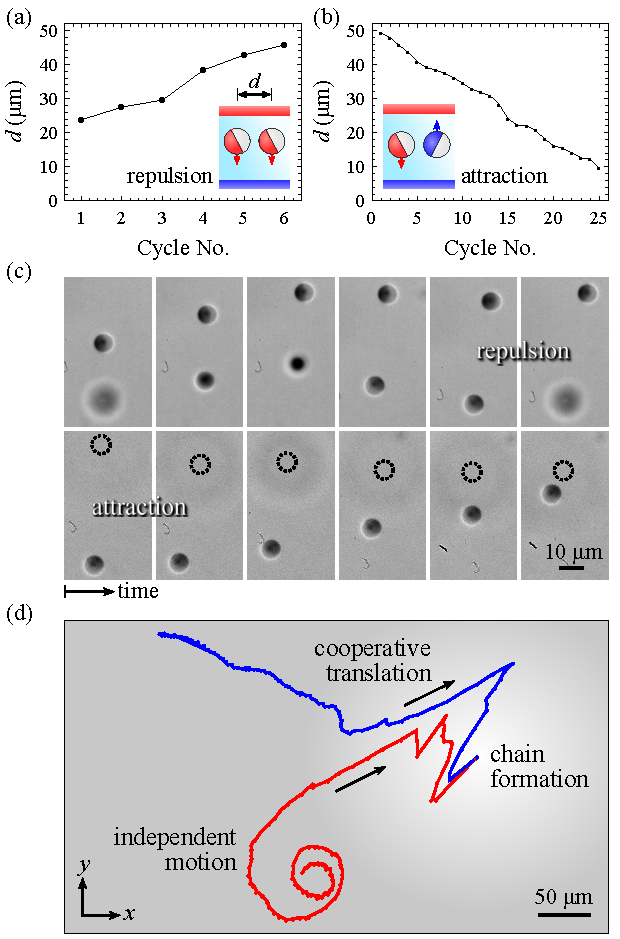
\includegraphics[width=10.5cm]{figures/2_5.pdf}
\caption{(a) The horizontal distance $d$ between two particles oscillating in phase increases during each oscillation cycle. (b) The distance between particles moving out of phase decreases each cycle. (c) Image sequence corresponding to data shown in (a) and (b). (d) Reconstructed trajectories for two interacting particles.  Initially, the particles are moving independently until their separation becomes less than the electrode spacing (here, $H=150~\mu\text{m}$). They then begin to move more quickly in a cooperative manner.  Ultimately, the particles come together to form an oscillating chain. See supporting video 5.}
\label{fig:5}
\end{figure}



%%%%%%%%%%%%%%%%%%%%%%%%%%%%%%
\section{Conclusions}

Contact charge electrophoresis drives the rapid oscillatory motion of conductive microparticles within nonpolar fluids.
Particle asymmetries can be used to rectify such oscillatory motions to achieve directed transport perpendicular to the applied field.
Rectified motions derive from particle rotations near the electrode surface upon contact charge transfer, which lead to repeated displacements in a common direction.
This type of self-propulsion exhibits several characteristics that distinguish it from related systems based on self-phoresis, induced-charge electrophoresis, or Quicke rotation.
Owing to the negligible electric currents through the nonpolar fluid, particle motions are highly efficient and require small energy inputs (ca.~1 nW / particle) \cite{drews2015contact}. 
Rapid particle motions can enhance microscale mixing within nonpolar fluids \cite{cartier2014microfluidic}, which could be harnessed to accelerate catalytic reactions limited by mass transfer.
Long-ranged electrostatic interactions among the particles results in complex collective motions relevant to the study of active matter.
Importantly, the directed CCEP motions of asymmetric particles can in principle be engineered by tuning the particle shape and surface composition.
The rational design of such active components is a critical prerequisite for constructing dynamic colloidal assemblies capable of useful functions -- that is, colloidal machines.


%%%%%%%%%%%%%%%%%%%%%%%%%%%%%%







